\documentclass[11pt,a4paper,oneside]{article}
\usepackage{fullpage}
\usepackage{hyperref}
\usepackage{amsmath}
\usepackage{comment}
\usepackage[pdftex]{graphicx}
\usepackage{url}
\usepackage[all]{xy}
\usepackage{caption}
\usepackage{subcaption}
\usepackage{chngpage}

\begin{document}
\title{\textbf{Dutch Nao Team}}
\author{\textbf{Technical Report 2012}\\ 
\url{http://www.dutchnaoteam.nl}\\\\
Faculty of Science, Universiteit van Amsterdam, The Netherlands}
\date{\today}
\maketitle

\begin{figure}[htb]    	
\centering
\fbox{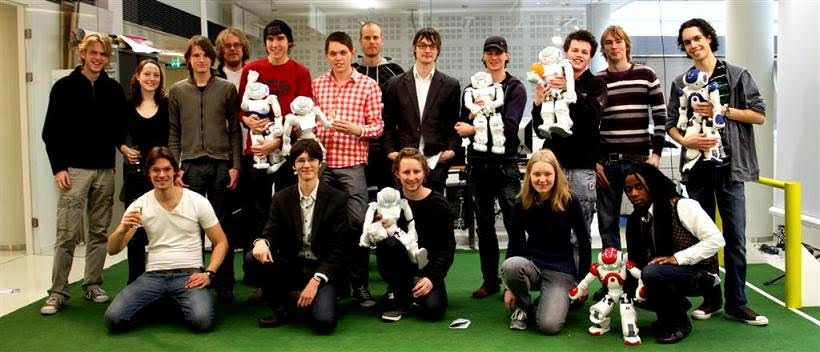
\includegraphics[width=1\columnwidth]{TeamLarge.jpg}}
%\caption{The Dutch Nao Team}
\label{fig:TeamPhoto}
\end{figure}

\begin{figure}[htb]    	
\centering

\includegraphics[width=0.3\columnwidth]{DNTLogo.png} % logo may look better when smaller
%
\includegraphics{DNTLogo.png} % real size of image
%\caption{The Dutch Nao Team Logo} % looks better without caption
\label{fig:DNTLogo}
\end{figure}

\newpage
\tableofcontents
\newpage
\section{Introduction}
The Dutch Nao Team consists of Artificial Intelligence students from the Universiteit van Amsterdam, supported by a senior staff-member. The Dutch Nao Team is the continuation of the Dutch Aibo Team; a cooperation of several Dutch universities who were active in the predecessor of the Standard Platform League \cite{AIBOTeam2006, AIBOTeam2005, AIBOTeam2004}. The Dutch Aibo Team has been successful, both in the competition and with a number of publications \cite{ArnoudJurgen2009, RoboticDog2008, Panoramic2007, ColorLearning2006, Localization2006, Perception2005}.
The Dutch Aibo Team always published their source-code online including a technical report about the innovations \cite{Visser2006}.
The Dutch Nao Team will continue this tradition. The Dutch Nao Team debuted in the SPL competition at the German Open 2010 \cite{DutchNaoTeamTDP2010}.\\

The responsibilities have this year been distributed over our team as follows:
\begin{description}
\item[Supervisor:] Dr. Arnoud Visser % (assistant professor Intelligent Systems Lab Amsterdam) %assistent professor is a combination of researcher and teacher
\item[Coordinator:] Duncan ten Velthuis
\item[Vice-coordinators:] Camiel Verschoor, Auke Wiggers
\item[Programmers:] Auke Wiggers, Chiel Kooijman, Hessel van der Molen, Inge
    Becht, Maarten de Jonge, Michael Cabot, Richard Pronk, Sander Nugteren,
    Tijmen Blankevoort, Erik van Egmond, Anna Keune
\item[Sponsors:] Placeholder
\end{description}

\section{Qualification}
This year the Dutch Nao Team made the commitment to travel to Mexico City for the RoboCup 2012. In December a qualification document \cite{DutchNaoTeamQualification} and qualification video\footnote{Available at \url{http://www.youtube.com/watch?v=laCXVb2dtPQ&list=PLCFE0DE27EB5C8C9D&index=1&feature=plpp_video}} were produced. The qualification document described the research that was to be performed in the upcoming months and how this was to be achieved.

\section{Competitions}

\subsection{Iran Open}
\begin{figure}[htb]    	
\centering
\fbox{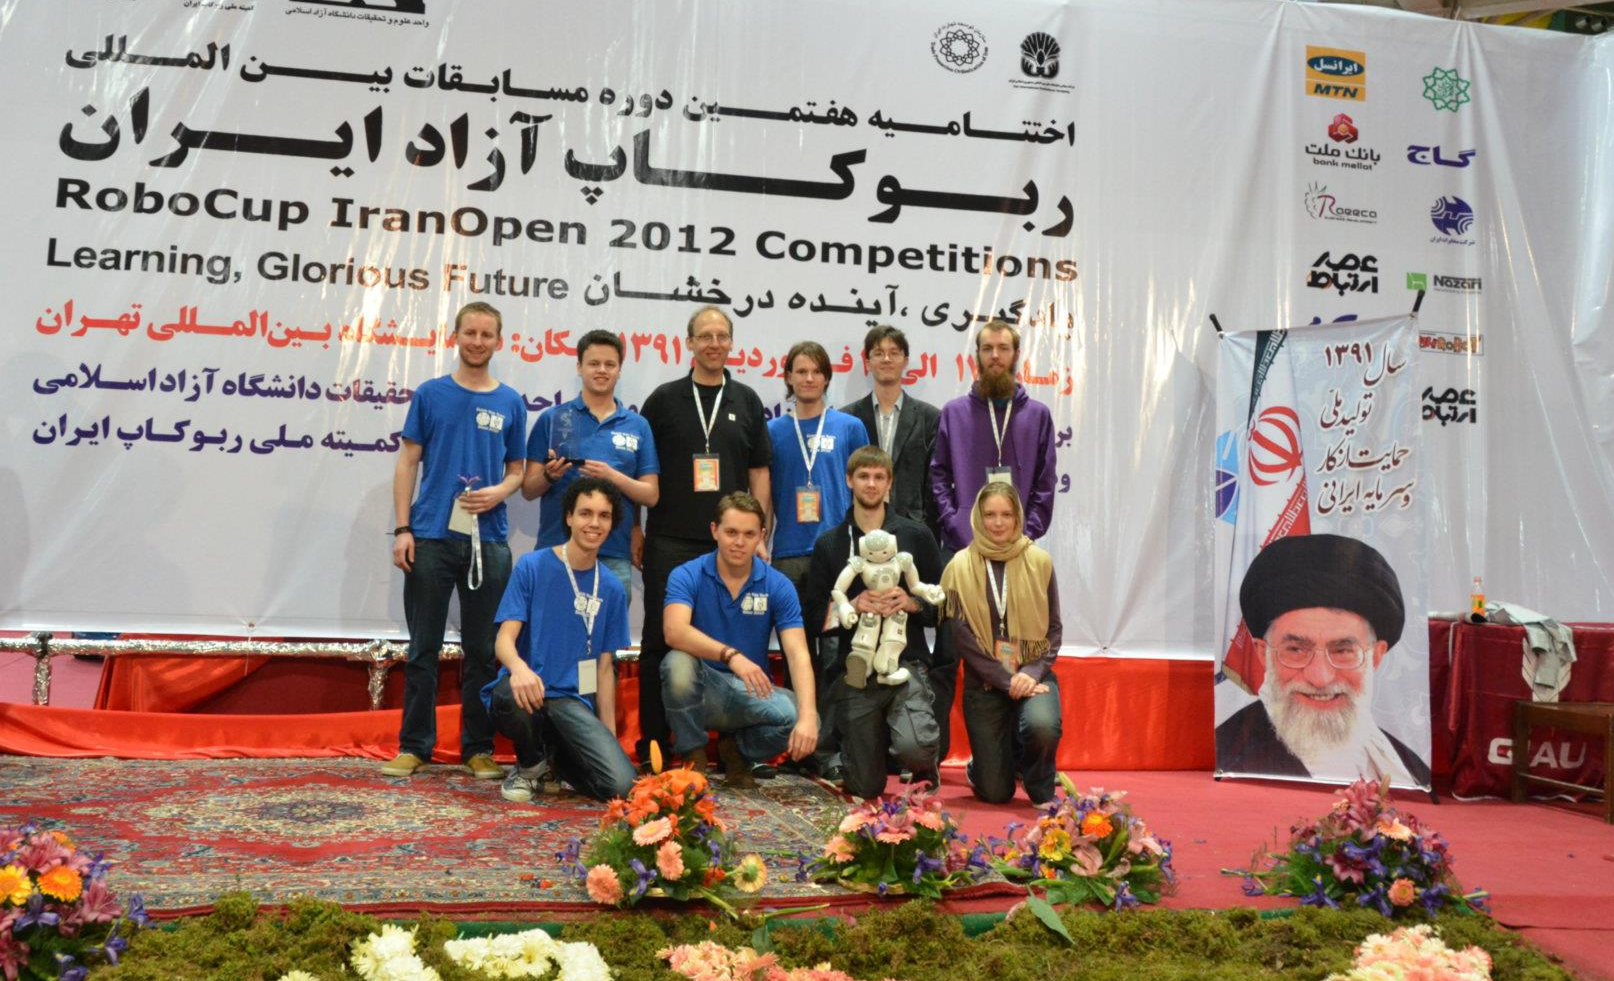
\includegraphics[width=0.5\columnwidth]{TeamPhotoTeheran.jpg}}
\caption{The Dutch Nao Team in Teheran}
\label{fig:TeamPhotoTeheran}
\end{figure}

A total of six teams competed in the Iran Open Standard Platform League:
\begin{enumerate}
\item AUTMan (Iran), first place
\item MRL (Iran), second place
\item Berlin United (Germany), shared third place
\item Dutch Nao Team, shared third place
\item Kouretes (Greece)
\item DreamwingSP
\end{enumerate}

\subsubsection{Matches}
In total 5 matches were played. Two matches were lost, with 0-6 to AUTMan and 0-2 to MRL. The match against Berlin United and Kourettes ended up in a tie (both 0-0), and the match against DreamingSP was won with 1-0.
The main problem in the competitions was with the vision. The Naos recognised a ball often outside of the field. The Naos also had problems with connection to the network so communication could not be tested in the matches.

\subsubsection{Developments}
Due to the above mentioned problems the first steps towards a calibration tool were made for simple color calibration, as well as a bounding box implementation so that the Naos no longer could find a ball outside of the field.

\subsubsection{Open Challenge}

For the Open Challenge multiple projects were presented that were worked on by members of the Dutch Nao Team, such as \ref{}\ref{}
The presentation ended up earning the third place of the open challende

\subsection{RoboCup Mexico}

Twenty-four teams from all over the world competed in the RoboCup 2011. We've played against a few of them:
\begin{enumerate}
\item rUNSwift, lost, 0-10
\item RoboCanes, won by distance in the penalty round
\item The Portugese team, match ended 1-1, lost by penalty round with 1-2
\end{enumerate}
The biggest problem faces in Mexico was the difficulty with connecting to the network (something every team had to try and cope with) but mostly the fact that the state of the code was not so it could be run easily, resulting in crashes of the robots.
\subsubsection{Developments}
A lot fo the time onely fixes were made to the already existing code.

\section{Program}
The program used in the RoboCup 2011 is written solely in Python. It is compatible with Python versions 2.61. OpenCV for Python is used, mainly for image processing. The files used are all original files written by members of the Dutch Nao Team. Different files are used for different sections, for instance, motions are all specified in a single file and not in the file containing the main program.
\subsection{Architecture}
\label{sec:architecture}
The program solves the game problem using a double state machine in the file \texttt{soul.py}. At the highest level are the \textit{states}, which are the game states as specified by the gamecontroller. 
At a lower level are the \textit{phases}, which are specific situations during a game. Transitions between the states and phases are made based on external input (conditions). 
For state-transtitions, the external input is a message from the GameController and/or the button interface (see section \ref{sec:communication}). 
For phase-transitions, the external input is based on observations (see section \ref{sec:vision}). 

%\begin{displaymath}
%    \xymatrix{								&	& \texttt{BallFound} \ar@/^/[ddll]^{\texttt{ball lost}}\ar@/^/[dddd]^{\texttt{ball close}} \\
%									&	&			\\
%	  \texttt{BallNotFound} \ar@/^/[uurr]^{\texttt{ball seen}}	&	&			\\
%              								&	&			\\
%									&	&\texttt{Kick}\ar@/^/[uull]^{\texttt{ball lost}}\ar@/^/[uuuu]^{\texttt{ball too far}}  			}
%\end{displaymath}

\begin{figure}
\centering
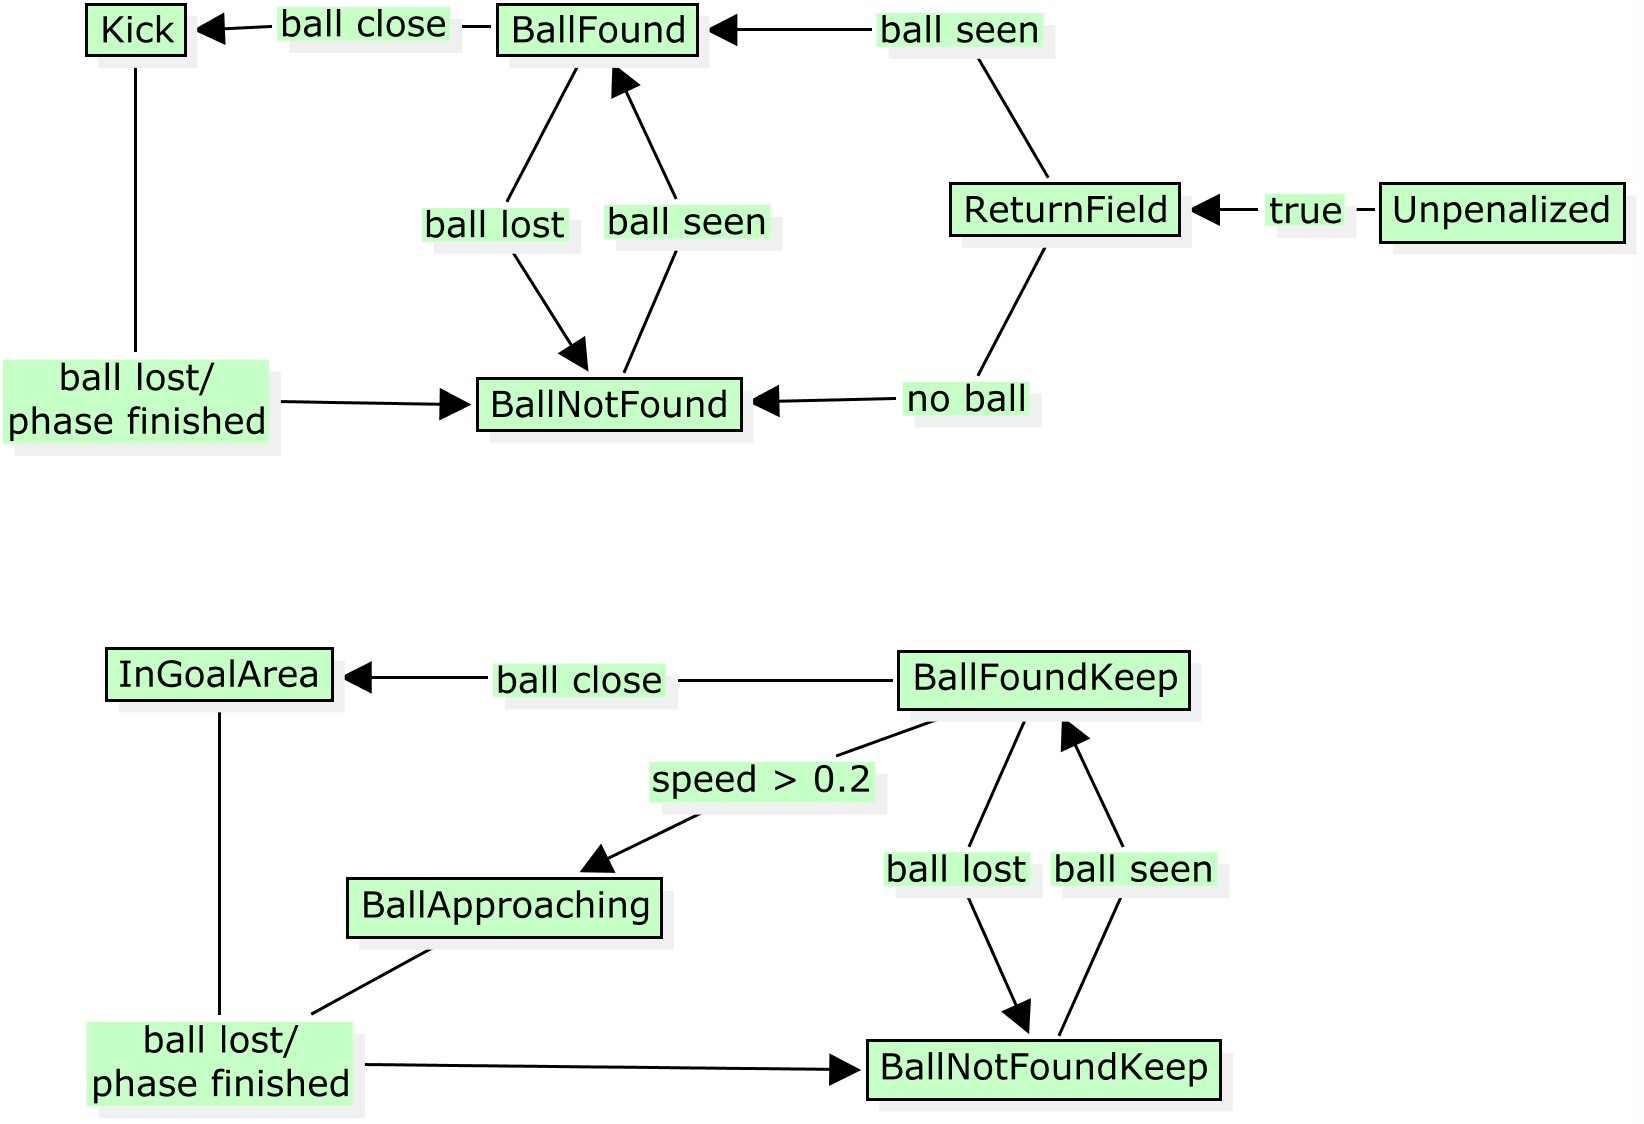
\includegraphics[width=12cm]{Conceptmaps.jpg}
\caption{The phases for both player (top) and keeper (bottom) and conditions for transition between phases.}
\label{fig:phases}
\end{figure}

In each of these phases, checks are made to see if conditions for transition are met (e.g. if in \texttt{BallFound} phase and ball close enough for a kick, go to \texttt{Kick} phase). An overview of these phases and conditions can be found in figure \ref{fig:phases}. An advantage of this approach is that the main problem, playing a game of soccer, is divided into smaller problems, which can be solved independently and locally. A second advantage is that phases can be tested without executing the entire program. In effect, the tests are less time-consuming. On the other hand, the Nao is not able to process circumstances that are not specified in a phase. The solution implemented is a straightforward one where phases can not be interrupted until they have finished. This would not, or less so, be the case if a single program covered the entire game problem. A short explanation of every phase in our program:\\\\
\textbf{BallFound} \\
Contains a findBall call to vision, which returns an x- and y-value representing the relative location of the ball (if found). Uses the found location to move Nao towards the ball. Transition conditions: Ball not found or ball close (close being close enough for a kick). How close this is depends on circumstances of the field (lighting changes interpretation of distance, how fast the Nao walks depends on the carpet, etc.) \\\\
\textbf{BallFoundKeep} \\
Similar to \texttt{BallFound}. The main differences are that the keeper does not walk towards the ball and that old positions of the ball are tracked as well. It is possible to derive speed and direction of the ball using these old positions and some geometry. If two or more positions are known, a function through these points $f(y)$ will intersect with the Nao's $y$-axis in $(y,0)$. The direction of the ball, which is the direction in which the Nao should dive, is determined by that specific $y$. An estimate of the speed at which the ball is moving towards the Nao ($x$-direction) is derived by taking two ballpositions and subtracting the $x$-positions. Transition conditions: Ball moving towards keeper (speed high enough) or ball close (low speed).\\\\
\textbf{BallNotFound} \\
When a player can not see the ball, the head moves around to scan for it. If, after a full scan, the ball is still not found, Nao turns around. Transition condition: Ball found.\\\\
\textbf{BallNotFoundKeep}\\
Similar to \texttt{BallNotFound}, the difference is that the keeper does not turn when a ball is not found. Transition condition: Ball found.\\\\
\textbf{Kick}\\
Player-only phase. Player is close to the ball and scans for goal. Player takes action if a goal is found, action depends on which goal is found. Angle towards goal is used as input for the kicking motion. Transition conditions: Ball lost or phase finished (ball kicked). A special transition was added later: If the ball somehow moves during the kick phase and is too far to kick, move to the BallFound phase.\\\\
\textbf{BallApproaching}\\
Keeper-only phase. Ball moves at high speed towards the keeper in a certain direction \texttt{dir}. Keeper takes action depending on \texttt{dir} (diving or sidestepping, left or right). Transition condition: Phase finished. \\\\
\textbf{InGoalArea}\\
Keeper-only phase. When the ball is in the goalarea, the keeper walks towards it, kicks it and walks back. As returning to the center of the goal is still impossible for us, this phase is not used in the current program.\\\\
\textbf{Unpenalized}\\
When a player or keeper is unpenalized, it moves to this phase first. It tells the player to walk 2 meters in x-direction (forward). Player/keeper then goes to phase ReturnField.\\\\
\textbf{ReturnField}\\
This phase can only be reached from the \texttt{Unpenalized} phase. While the player is walking, search the ball. Transition conditions: Ball found or end of walk.\\

Keepers behave differently from other players in the field. Therefore, a similar approach is used but with different names for the phases (e.g. \texttt{BallFoundKeep} instead of \texttt{BallFound}). This shows another disadvantage of our approach: When a bug is found or a change is made in the phases for regular players, it has to be changed twice, once for the normal phases and once for the keeper phases. However, different behaviour for the player and keeper can be made, where this is needed (e.g. emphasize movement along y-axis for keeper to protect the correct side of the goal, whereas a player will emphasize movement along the x-axis to reach the ball faster). A phase contains the following: 
\begin{itemize}
\item A call to receive visual information and, if needed, further processing of this information
\item One or more condition checks for transition to other phases
\item One or more motion calls
\item Optional: print statements for debugging purposes
\end{itemize}
The exception to this is the \texttt{Unpenalized} phase. This phase cannot be reached from any other phase when in the \texttt{Playing} state and it does not ask for visual input. It is reached when a player or keeper was in the \texttt{Penalized} state and is unpenalized. Its sole purpose is to make this player then walk two metres forward (in the direction it is facing, this should be towards the field) and thus prevent it from staying at the sideline. 

As each phase is implemented as a Python function, it can be called independently. The system thus works as a loop calling the function corresponding to a game phase. It should be noted that the phase can be changed in any state but the corresponding function is only called in the Playing state. Also, a keeper that is penalized will reach the \texttt{Unpenalized} and \texttt{ReturnField} phase successively, meaning it turns into a regular player after being penalized.  

Calls to other aspects of the program (vision and motion) are made through interfaces. These interfaces are specified in different files. DNT chose to use this approach instead of regular motion calls to make the main program (\texttt{soul}) easier to understand. An example: Function \texttt{StandUp()} in \texttt{motionInterface.py} checks the pose of the Nao and then takes action corresponding to this pose. Instead of checking the pose in the main program, this entire process is specified in a different file and can be initiated with a simple function call. 

\subsection{Vision}
\label{sec:vision}
% Michael
The ball- and goal-detection are based on color filters. Prior to a match calibration is needed to set the HSV-color-ranges of the red ball, yellow goal and blue goal. These ranges are then used to filter the image taken by the Nao resulting in a grayscale image. When detecting the ball the filtered image is smoothed to remove any noise. If the brightest pixel passes a threshold then this is assumed to be the ball. The position of the ball is calculated by projecting that pixel onto the ground using the location and orientation of the camera when the snapshot was taken. A small improvement of this ball tracking algorithm of last year is the use of bounding boxes to prevent searching the ball outside of the playing field, by filtering on the color of green (figure \ref{fig:boundbox_ball} shows this smalle improvement). 

\begin{figure}[htb]    	
\centering
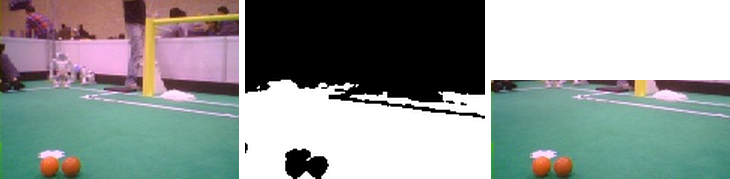
\includegraphics[width=0.8\columnwidth]{boundbox.png} % logo may look better when smaller
%
\includegraphics{DNTLogo.png} % real size of image
\caption{Using a bounding box approach to minimize the ball search space} % looks better without caption
\label{fig:boundbox_ball}
\end{figure}

This prevents that the Nao will find the ball outside of the field and in environmental noise(which has been often the case in previous matches).

The goal is detected by appending vertical lines in the filtered image to form blobs. These blobs are tested to see if any describes a goalpost. If two posts are found then the angle towards the goal is calculated.

All the vision components were set up so to run parallel with each other. This was removed in the latest release of the program to prevent overheating of the Nao's head.  

\subsubsection{Blob and Nao detection}
In order to recognize features of the environment, a scan is done for blobs of colour in the snapshots the Naos make while walking. To do this, first each picture is corrected for varying lighting conditions. This is done by taking a sample snapshot and finding the pixel that most approximates white. Luckily, since the robots are playing a game of soccer, there will almost always be a white field line somewhere in the snapshot for sampling. The white point is then assumed to be white and all other colors are corrected to make this pure white. This will give consistently coloured snapshots to work with.

Then, the pictures are scanned for colours in a certain range (for example, yellowish colours for the yellow goal). These color ranges are pre-set according to tests, due to correcting these colours, the pictures are consistent enough to make this assumption. A new black and white picture is made representing this scan, with white pixels denoting a positive pixel and black denoting a negative. This gives a black image with the shape of the object that is scanned for in white, and usually some noise. Then each line of the image is checked for lines of one or more white pixels. These pixels represent a blob on a certain line, line blobs. The data on all of these line blobs is stored along with a unique ID value. Due to this line blobs can be easily re used.

Once the entire image is scanned, this will result in a database filled with line blobs. The next step is to convert these line blobs into two-dimensional blobs. This is done by looping over all the line blobs and checking if any of the line blobs, on a line below the current line, are within the horizontal range of the current line blob. If this is the case these line blobs are mapped to one ID value. Once this is done, all the blobs with the same ID are found and the new maximum edges are calculated. This is stored as a new blob with a new ID, along with this data.

To detect a Nao, all insignificantly sized blobs are discarded; this filters most of the less significant noise. Sometimes, faraway Naos are also discarded during this step; however, this is not a real problem since opponents this far from our goal are no immediate threat. This does leave the bigger noise groups in the picture. To determine which of these objects are actual Naos, a check is done on three lines above and two below each blob. If the detected blob does indeed belong to a Nao, each of these lines should be (approximately) white.

\subsubsection{Goal Recognition Algorithm}
\label{sec:goalrecognition}
The following algorithm is based on the shape of the goal. The goal is defined by its two poles. The poles in the image are rectangular with a length and a width defined by thresholds. Goal recognition is performed on a color filtered image. The color can be either blue or yellow. In short, to check if the poles are present, the algorithm searches the image in vertical direction for lines long enough to be poles. Then it checks if the lines are adjacent and the width is wide enough to be a goal.\\\\ 
Algorithm step-by-step (the threshold $t$ is 20)
\begin{itemize}
\item Filter the image based on color.
	\begin{itemize}
	\item Form a dict of vertical lines.
	\item Iterate from top down steps of ten ($0.5t$) pixels, start at ten.
	\item When a true pixel is found go back nine ($0.5t-1$) pixels (remember the step of ten).
	\item Start iterating by one pixel until a true pixel is found.
	\item Then count until twenty ($t$) pixels are found in a row or until a false pixel is found.
	\item When a false pixel is found retry at the last known pixel (ten ($0.5t$) further).
	\item When a true pixel is found do the same but bottom up .
	\item Remember starting and ending pixel.
	\item If no pixels is found there is no need to start from bottom up.
	\item Bottom up searching cannot go past the starting pixel.
	\end{itemize}
\item Group the vertical lines together.
	\begin{itemize}
	\item Iterate from left to right.
	\item If the left and right one are adjacent and do not differ in length by more than 50\%
	\item If a group is found and large enough remember it and find another group.
	\item Return the two largest groups.
	\end{itemize}
\end{itemize}

\subsection{Motion}
The first steps towards designing a dynamic kick were made this year. A multiple of
modules have been constructed to solve this problem \cite{Becht2012}.
Using a  forward kinematics module it now is possible to 
find the position of a limp relative to one of the legs. This forward
kinematics module also gives the possibility to locate the Center of Mass and
is used in a Center of Mass based P-controller to keep the Center of Mass above the
Support Polygon. A second balancer uses online data in the foot sensors to correct outside interferences from other Naos during a competition. 

Another critical part of dynamic motion that has been mastered is the Inverse Kinematics. This has been approached by the damped least squares method, in which the desired position is approached over multiple iterations. Due to time constraints the module is written in C++ instead of our usual Python but uses a Python SWIG wrapper to easily communicate with the rest of the Python code.
 
At the moment all of the motions used in matches are still keyframe motions. The kick and back kick are given an angle (angle to the goal) as input. The result is an open-loop motion kicking the ball in the specified angle. The keeper movements are of our own design. We use the walk engine by Aldebaran which is a stable omnidirectional walk. Get-up motions are improved versions of the motions provided in Choreographe.


\subsection{Communication}
\label{sec:communication}
% Sander en Erik, over de gamecontroller (copied Sander's contribution of July27 from GoogleDoc)
At first, the program was tuned to listen to a specific IP address. It would receive the input stream, parse it, and store the information in a GameController object. Recieving the data was done by the \textit{refresh()} method, and the object had several get methods to acquire the data from the object. The refresh method returned true if it had recieved data, and false if it hadn't.

In the Rome Open, the program was made to display the right LED’s on the chest and feet, depending on the current team color and the game state (green for playing, red for penalized, etc.). 

After the Rome Open, the button interface was implemented and combined with the game controller to make a state controller. This is a threaded module which is called to get the game state according to the buttons and game controller (if game controller is present).

Furthermore, the \textit{controlledRefresh} method was implemented, which calls the refresh method repeatedly during a specified interval to see if the game controller is still online (default 4 seconds). If it is, it returns true. If the connection timed out, it returns false, and the state controller starts listening to the buttoninterface, before trying to connect with the game controller again.

In Istanbul it occured, that some teams were broadcasting their own game controllers on the same IP address, which caused problems as the program would listen to all of them. The solution to this was making the program listen to game controllers broadcasting a match with our team number in it only.  

Communication between Naos has been proven to work successfully using built-in methods provided by Aldebaran. It is possible to store a string in memory of a Nao. Other Nao's can receive this specific string if the IP adress is known. This communication will be used to `tell' other Naos how close to the ball they are. Visual information, once processed, can be sent through use of a (not yet determined) protocol, e.g. 'Ball 0.500 0.300 0.583' would mean a ball is at relative position (0.5, 0.3) at distance 0.583 meters.

\subsection{File architecture}
\begin{figure}[htb]    	
\centering
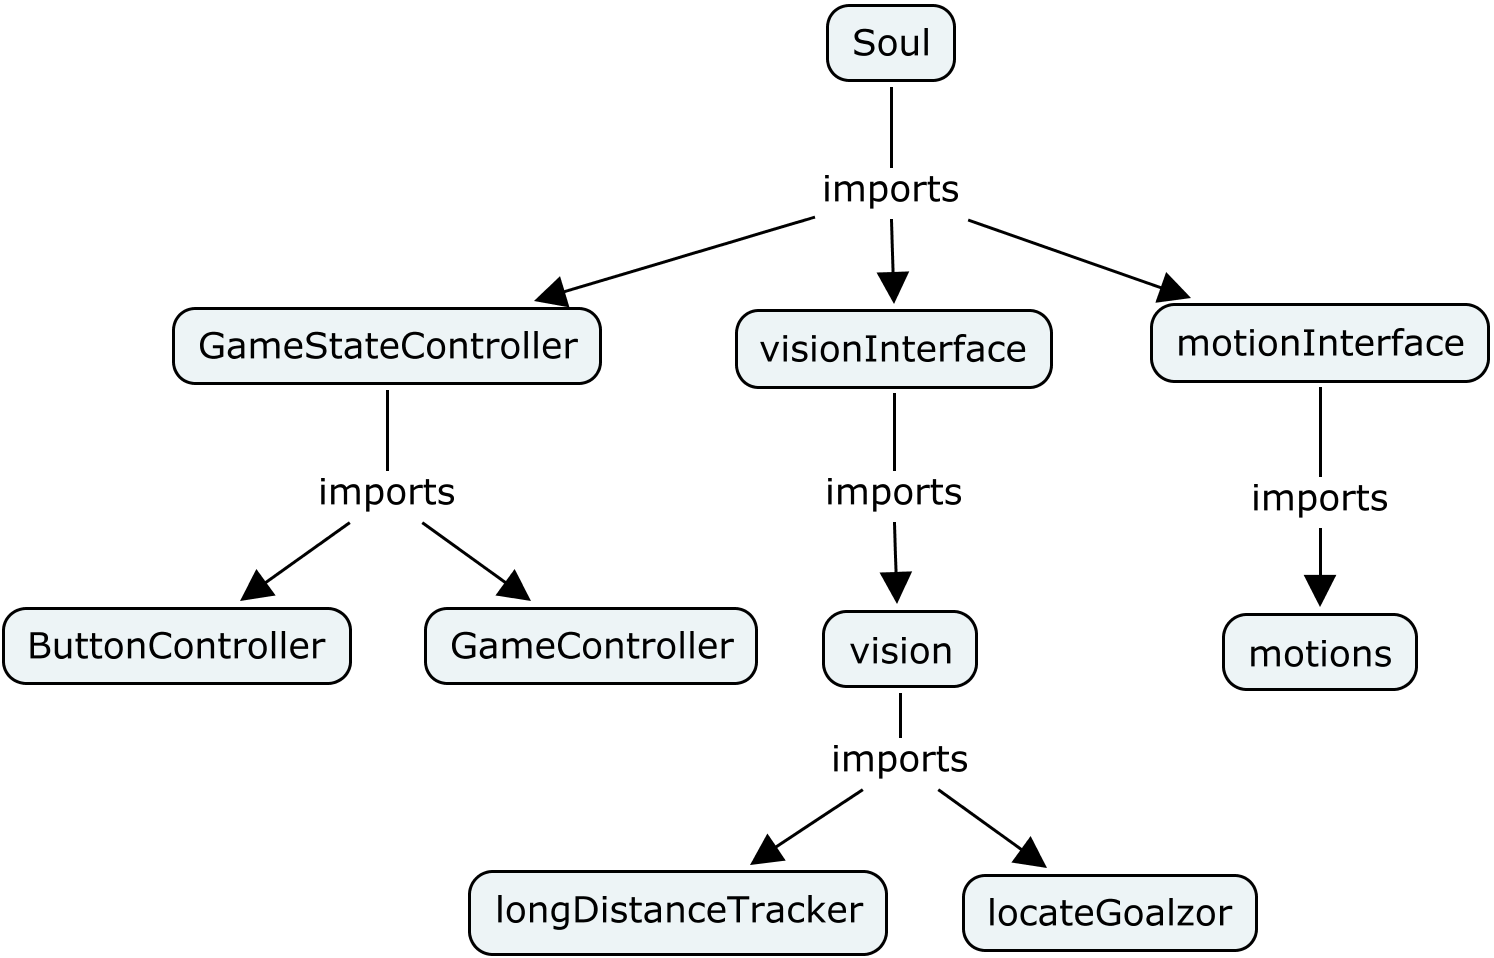
\includegraphics[width=0.7\columnwidth]{cmapFiles.png}
\caption{Hierarchy of files as used in the RoboCup 2011}
\label{fig:File}
\end{figure}
The file hierarchy (see figure \ref{fig:File}) that is used prevents the main program (\texttt{soul.py}) from becoming a chaos. The contents of the files are described in more detail in Appendix~\ref{app:file_overview}.
Motions are specified in a single file. 
For different visual tasks, different files are used. This is mainly to make testing easier (tasks can be tested and programs can be altered simultaneously without trouble due to incompatible versions). 
To make matters even easier, interfaces (\texttt{motionInterface} and \texttt{visionInterface}) are used. These interfaces are used because almost every vision task starts with a snapshot and conversion of this image. 
It would not be aesthetically pleasing to make these function calls in the main program every time a vision call is made. 
The vision interface is well used; the motion interface is implemented merely for completeness (as vision is comparable to motion, both are straightforward tasks that do not alter the flow of the main program directly, unlike the game controller and button interface). The game controller and button interface are each specified in a file to make testing and altering individual functions easier.


%Removed localisation... Should be added?

\subsection{Simulation}

At the Universiteit van Amsterdam a physical realistic model of an Aldebaran Nao robot inside the simulation environment USARsim \cite{Carpin2007icra} is developed. A major advantage of this simulator is that uses the local installation of NaoQiSDK to process commands to the Nao robot, which means that the same python code can be used for the real robot and the simulated robot. 

It was even considered to use a NaoQi system image inside a virtual machine to circumvent the usage of a local NaoQiSDK, but private discussions with Aldebaran employees\footnote{Manuel Rolland and Cedric Gestes} on the RoboCup revealed that Aldeberan itself is busy with this development for their open source release in Fall 2011. 

USARsim is a simulation environment based on the Unreal Engine, which enables easily modification of the environment around the robot (in contrast with Cogmation's NaoSim) and create realistic lighting condition.  

In the previous version of USARsim (based on UT2004) a wide variety of robot models was available, including a Sony Qrio and Aibo. The model of the Nao robot is the first type of walking robot in the new version (based on Unreal Development Kit).  

First a Nao model with two joints (T2) was developed, which was gradually upgraded to a model with 21 joints (T21). The different parts are now nicely scaled, as illustrated in Fig.~\ref{fig:nao_scaled}.

\begin{figure}[hbt]        
\centering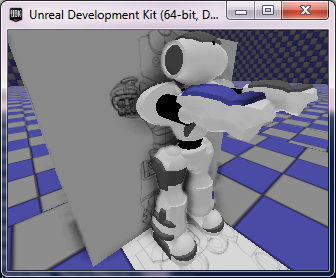
\includegraphics[width=.5\columnwidth]{nao33_correctheight.png}
\caption{A model of an Aldebaran Nao robot in USARsim, including a scaled drawing from the Aldebaran documentation}\label{fig:nao_scaled}
\end{figure}

Important for a physical realistic simulation is the calibration of the joints' dynamic behaviors. The dynamic behaviors are configured with parameters such as the mass distribution, the inertia and the gravity. 

Several tests related with gravity, forces and constraints have been performed to validate basic assumptions about the physics of the simulated world. A nice feature of the UDK-model is that the double constraint for the HipYawPitch joint is seemlessly incorporated into the model.

With the center of mass close to the hip, representing a mass distribution according to Aldebaran's specifications, the robot currently can stand up and sit-down. Even more complex behaviors as the Tai Chi and Thriller dance can be executed without loosing balance.

Currently the walking behavior is fine tuned by letting the real and simulated robot walk an eight shaped figure. In the near future the complexity of the tests will be increased, including more complex movements of the Dutch Nao Team.

The development of this open source simulation of a Nao robot not only valuable inside the Standard Platform League, but should also be interesting for the Soccer Simulation League and the @ Home League. Outside the RoboCup community this simulation could be valuable for Human-Robot Interaction research.

\subsection{Tools}
Some various tools have been developed to ease preparation before a match. 

\subsubsection{Calibation Tool}
One thing that proved to be a problem in tournaments was color calibration. Previously this was done manually by taking samples of an image and kind of estimating what the color range would be. This led to a lot of inaccuracy and difficulty in finding the ball and goalposts. This has been alleviated with a graphical calibration tool written in C++ with Qt. It allows the user to load an image and select an area, either through dragging rectangles or a magic wand tool. It then ouputs the HSV range (minimum and maximum values for the hue, saturation and value) of the select area(s) (see image \ref{fig:calibrationtool}).

\subsubsection{Preparation Script}
To ease the preparation for a match, a Python script has been made to find all Nao robots on the network using Avahi and automatically push code and a generated naoinfo.txt. 

\section{Installation Guide}
\subsection{Requirements}
\subsubsection{Program}
The following items are required to run our program \texttt{soul.py}:
\begin{itemize}
\item Nao
\item NaoQi 1.10.52
\item Computer (Windows/Linux)
\item Secure Shell Client (Windows) / SSH (Linux)
\item TurtoiseSVN (Windows) / SVN (Linux)
\item Link to repository\footnote{\url{http://code.google.com/p/dnt-rules/}}
\end{itemize}

\subsubsection{Simulation}
The simulation environment consist of two parts: UsarSim which represents the SoccerField (or another world) where one or multiple robots can be spawned and UsarNaoQi which represents the robot (and translates NaoQi commands into usarsim commands).
For UsarSim an installation guide is available\footnote{\url{http://sourceforge.net/apps/mediawiki/usarsim/index.php?title=Installation}}. For UsarNaoQi an usage guide is available\footnote{\url{http://nao.sandern.com/doku.php?id=usage}}.

The UDK version of UsarSim can be downloaded from sourceforge with the command \texttt{git clone git://usarsim.git.sourceforge.net/gitroot/usarsim/usarsim}, for instance from a Cygwin shell. To allow the usage of the two cameras of the Nao a tool is needed, which is (not yet) available
under git. An update of this tool which uses the video hook (EasyHook) native to UDK to get access of the camera images is available for download\footnote{\url{http://nao.sandern.com/downloads/ImageServer_Beta3.zip}}. This tool should be installed in the directory USARTools.

UsarNaoQi is available for download at \url{http://svn.sandern.com/nao/trunk/usarnaoqi}. The code requires an installation of Visual Studio 2008 and an installation of NaoQiSDK. The location of the NaoQiSDK installation should be specified in the environment variable \texttt{AL\_DIR}.

The latest version of UsarNaoQi is tested with NaoQiSDK 1.10.52.

\subsection{Guide}
\subsubsection{Program}
Follow these steps to install and run the program \texttt{soul.py}:
\begin{enumerate}
\item Download the program from our repository with a SVN program.
\item Move downloaded files from the previous location to the home folder of the Nao (Linux environment).
\item Navigate to folder `home\textbackslash naoinfo' (Windows) or `/home/naoinfo/' (Linux). 
\item Create a file `naoinfo.txt', line 1 is the playernumber, line 2 the teamnumber. Line 1 should be 1 if Nao is a keeper.
\item Navigate to `home\textbackslash naoqi\textbackslash lib' (Windows) or `/home/naoqi/lib' (Linux)
\item Call `python loader.py' from command line.
\item Nao will say that you have to press a footbumper to initiate football mode. Press the bumper.
\end{enumerate}
In this release, there is no safe way to stop the program. Rebooting the Nao or forcing a stop in command line both work but are not pretty solutions to the problem.

\subsubsection{Simulation}
To start the UsarSim including support for the cameras the following command should be given from the UDK directory: \texttt{Binaries\textbackslash Win64\textbackslash udk.exe RoboSoccer?game=USARBotAPI.ImageServerGame -log -d3d11"}.

\begin{figure}[htb]        
\centering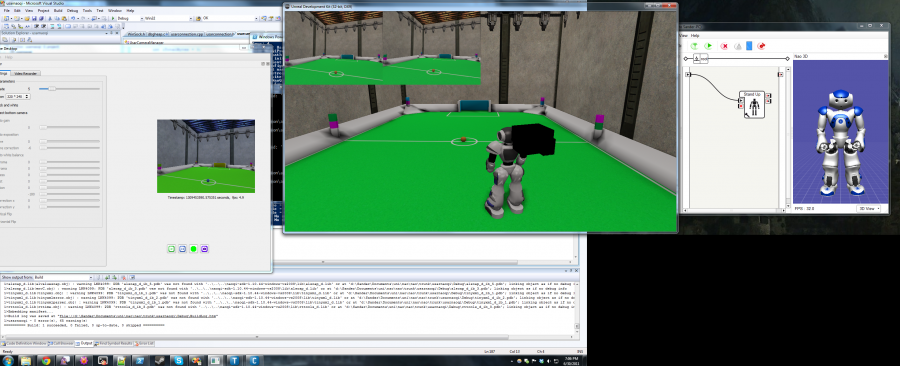
\includegraphics[width=.95\columnwidth]{NaoWithTwoCamerasInSoccerWorld.png}
\caption{The  Nao robot in the RoboSoccer environment of USARsim, including the view of both cameras in the upper left corner.}\label{fig:nao_robosoccer}
\end{figure}

To spawn a Nao in this RoboSoccer environment the command \texttt{usarnaoqi.exe} should be given. This program loads its default configuration from the file defaultconfig.xml.

The robot can now be controlled and monitored by any control program, including Aldebaran's Choregraphe and TelePathe (see Fig.~\ref{fig:nao_robosoccer}). The Nao is visible with the default name 'UsarSim1' in the connection windows of both Aldebaran programs.

The simulated robot can also be controlled with the Dutch Nao Team software by typing \texttt{python loader.py} on the commandline.

\section{Sponsors}
The Dutch Nao Team consists of students and most of them do not have enough money to pay for the travel to the Open competitions or the World RoboCup. Therefore, it is essential to get some sponsors. There are many companies that are eager to get some brand awareness and they are prepared to pay for it. It costs time and energy to find the right people from the right companies, but if it is done well, it might lead to a fine collaboration.

\subsection{Preparations}
There are a few things that the team needs to make some decisions on, before somebody starts contacting companies. Firstly, its necessary to know what the team has to offer; banner on the team's website, logo on the t-shirts or on the Nao's etc... Secondly, when the list is ready with all the possibilities that a company may use, prices for the individual options have to be determined. Sometimes people may ask whether there are packages (a few options packed together for a better price) that can be bought. Therefore, it is recommended to make some small packages (consisting of two or three options) for an attractive price, some normal packages and one large package, which contains everything that is offered by the team. This is due to the fact that every company has a different amount of money that they can spend on sponsoring. A larger company may be willing to pay more in contrary with smaller companies, that will try to get a better deal. After making the packages it is recommended to prepare some contracts. This is to prevent that the company has to wait.  It is up to the person who takes care of the sponsoring to know whether to go along with the negotiations or not. When the company is very small, they will not be able to pay as much money as the other companies, but every amount can be helpful fot the team. So it is good to consider your decision about the sponsor.

Another task is to find the companies that might be interested in sponsoring the team. The first choices should be Information Technology (IT) companies, because those are the companies that are primiraly looking for IT students. The internet is the best place to look for them and also to find another businesses that might want to collaborate with the team.

\subsection{Contacting companies}
When all the preparations are finished one can start contacting the companies that have been found. It is highly recommended that every company communicates with one person. This in order to prevent double deals. It also looks unprofessional if more than one person try to contact one person in a company. When a company is interested one should negotiate about what the company wants exactly. Then the contract can be set up and signed.

\section{Public Relations}
\subsection{Getting started}
The Dutch Nao Team is one year old now, which means the Public Relations (PR) department started from scratch, with no script, site or reference to a tournament the Dutch Nao Team had participated in. First of all, the team started with the most general concern of PR: launching the website. Given a website should appeal to a wide variety of people so it should not only describe technical terms, but also introduce the RoboCup and ourselves on a basic level. In addition, the site had to be a clear and easy to use, so everyone can find what they are looking for. To achieve this, a simple menu was made based on the subjects one might wonder about. Furthermore, the language of the site was English instead of Dutch, because of the international character of the RoboCup competition.

Secondly, the communication advisor of the UvA, drs. M. van de Laar, was contacted, who came up with a general script voor PR, which is described in the following section.

\subsection{Making the script}
\subsubsection{The script in general}
Public Relations is all about improving reputation and image. To achieve this, you will need a script revolving the following questions:
\begin{itemize}
\item Audience: Who does the team want to reach?
\item Objective: What does the team want to achieve?
\item Message: What does the team want to communicate?
\end{itemize}

\subsubsection{Audience}
The RoboCup is not very well known outside the robotics community, therefore, choosing a target audience was difficult. The goal was to reach (prospective) students in the teams field to show the possibilities of robotics and perhaps even to recruit new members. Another goal was to promote the RoboCup in general to a bigger audience. The team wanted to address the latter because it would help reaching prospective students and perhaps even sponsors. It was also important to keep the robotics section of the UvA up to date, because without them there would not even be the RoboLab.

\subsubsection{Objective}
In the Netherlands only a few people are familiar with the competition. The objective is thus to promote the reputation of the DNT and promoting the RoboCup. However, it is neither the task nor the responsibility of the DNT to provide a campaign for the RoboCup in general. Nonetheless, the ignorance is something to keep in mind when promoting the team.

\subsubsection{Message}
In short, the message for every group, comes down to:
\begin{itemize}
\item (Prospective) Students: See what the Dutch Nao Team does in their field and join!
\item Public in general: Learn about the possibilities of robotics!
\item UvA: Follow the progress of the team!
\end{itemize}

\subsection{Achievements}
For the past year we have mainly been working on the website and a general view of PR. The biggest obstacle was to decide where to start. Trying to reach our entire audience at once was too much to handle and on top of that we needed different approaches for each one.
\begin{itemize}
\item For our junior prospective students we gave a demonstration at the RoboCup Junior in science center NEMO. This was done to show youngsters the possibilities of robotics.
\item During the RoboCup tournaments everybody wore printed t-shirts to promote the team and improve our reputation within the league. 
\item At the Science Park there were posters of the Dutch Nao Team with information about us, our demonstrations, our progress and of course a reference to our website!
\item To keep contact with our supporters a Facebook-page and a Twitter-account were made. Through these, people from all over the world can follow our progress, thoughts and experiences.
\item And finally, to address the bigger audience, we made a press release about the participation of the DNT in the World RoboCup in Istanbul. We chose this event for the press release because a world cup generally is newsworthy for its international character. This particular press release can be found in Appendix~\ref{app:press_release}.
\end{itemize}

\subsection{Points of improvement for next year}
Next year it would be very wise to start with expanding the script to a much more detailed version. Last year we fiddled about for too long because our ideas were not specific enough and also: sending general messages to an unspecific audience is not efficient or functional at all. 

In addition, the goal to promote the reputation of the RoboCup in general is a job on its own, so it is something to bear in mind when you are writing to people outside the robotics community, but it is definitely not up to us to manage their PR!

On top of the press releases and emails, it is time to make a new, more professional website now that we have finally accomplished something and want it to last.

Furthermore, it is a new years resolution to attend more events for speeches as well as demonstrations.
And last, but not least, we would like to refer to the following site: \url{http://www.freepublicity.nu/}. Unfortunately we ran across this website at the end of this past year, but you can find lots of tips and trics there for the PR department.

\section{Travel}
The Dutch Nao Team travelled this year to Iran and Mexico to participate in competitions. For every journey, several arrangements had been made. This section describes, which arrangements were made.

%\subsection{Rome}
% The people participated did not want to share their travel experience and preparations

\subsection{Teheran}
This was a special journey as the Dutch Nao Team got invited by the organizing party (Qazvin University) and the costs for travel and stay were fully covered by them. Therefore, only the flight had to be booked and a visa had to be requested. It is important to do these two on time as both require some time. For the visa, the required documents have to be sent to the organizing committee, which will respond to you when the visa can be requested at the consulate in Den Haag. The organizing committee will make an official invitation letter for the participating members. To request the visa in Den Haag all participating members have to be present at the consulate. Requesting a visa can take up to one day. The flight was booked after a confirmation of the organizing committee was received. Before leaving, a document~\cite{Verschoor2012Iran} of all important facts about the country was sent to all participating members. This was to make sure that participating members were informed about the background of the country, possible required vaccinations, laws and uses of the inhabitants and advice about staying in the country. In Iran, the stay, transport, food, tours of the city were all organized by the committee. 

\subsection{Mexico}
This journey was to the RoboCup2012 where all international teams participated in a robot football World Cup tournament. The flight and hotel were booked quite late causing the price of the flight to be higher. A nice hotel was found nearby the location of the event (name of the hotel is El Diplomatico (located near the World Trade Center where the RoboCup was held). Breakfast and lunch was bought from the nearby supermarket. Dinner was bought and consumed at nearby restaurants. We traveled mostly by foot to the Robocup revenue, and sometimges using public transport. The first week of the journey was spend sightseeing around Mexico-city.

\subsection{Tips for the next journey}
This section describes the advice to the organizers of next year. The following points are important to take into account for next year:
\begin{itemize}
\item Have strict deadlines for participating students. Pay and sign up deadlines are both important as without money you cannot book the flight and hotel.
\item Start on time with booking the flight to reduce costs.
\item Find a hostel/hotel near the location of the event.
\item Write a travel information document. So all the important information bundled together.
\item Communicate clearly with the students participating in the team.
\end{itemize}

\section{Management}

\subsection{Season 2010-2011}
At the start of the project, the Dutch Nao Team (DNT) was split into different groups: {\it Vision}, {\it Motion}, {\it Communication} and {\it Architecture}. Each group consisted of a captain and sufficient members to complete their work. The captains were in control of the groups, as well as being a programmer. Above the captains were two other positions, the manager and advisor. Since the team was large at first, splitting the team seemed like a good idea at the time. It did work because the team started from scratch and had many work to do. After some time, this did not go so well. It became clear that the groups were dividing the DNT by blaming each other for bugs, loss of files and other complications. It also seemed that each group saw itself as a standalone group instead of cooperating with the rest of the team.
Halfway through the year, this setup was changed. Pairs were formed, which would then work on a single task (e.g. goal recognition, motion). These pairs worked independently and would add their programs only when finished. We also switched from Dropbox to SVN, a huge improvement which made the management of files easier (and tidier as well). 

\subsection{Season 2011-2012}
The major problem with participation last year was that it was voluntary, this made it hard to demand progress when someone was behind on his work. The second year there will only be members in the team that contribute actively. If anyone outside the team wants to help or contribute to the RoboCup through related work they still can but that will be either on minor projects that do not have a deadline or by helping existing pairs. Members that are unable to do the minimal required work for an extended period of time will have to talk with the manager and advisor, who will decide if a person can stay or has to leave the Dutch Nao Team..

A second problem was that the team started as a large group (23 people). As everyone, at that point, lacked experience in managing, the focus lies on keeping the team small. This makes management and organization easier and everyone in the team will feel more involved.  

\subsection{RoboCup Junior/Dutch Nao Demo Day}
On May 28th, the DNT had a small stand at the RoboCup Junior at NEMO, where the most recent code was showed off, by letting Naos play soccer on a small pitch which was open for public throughout the day. In collaboration with Dutch Nao Day a small demonstration was given.
 
The goal of the Dutch Nao Demo Day is to bring different Nao-owners that live in the Netherlands together, show each other the demonstrations created in the different institutes in the Netherlands and create - in a shared effort - one big demonstration, which is shown at the end of the day in the theatre of the science center NEMO. This was and (will hopefully remain) an excellent opportunity to show the efforts of the Dutch Nao Team to the public. 

\section{Evaluation and Future Improvements}

The Dutch Nao Teams second year has made some progress from the previous year. The first steps towards closed loop motions has been explored, although not yet implemented into the code at this point. Some tools were developed to ease the setup before a game, making it less of a hassle to ready the Naos before the match.

\subsection{Future work}
The Dutch Nao Team would like to further develop clodes loop motions, either by making a closed loop gait or create a fully dynamic kick. Falling during a kick was one of the main problems in this years RoboCup. A faster gait would be an important improvement because this teams robots are currently the slowest in the competition.

Further the idea of rewriting all code into C++ is a possibility.

Line detection was not further explored this year, but would be a good to add to the arsenal.


\subsubsection{Line Detection}
To find a line on the field, an image is filtered on white pixels (lines are white). In this filtered image, the Houghlines algorithm, found in OpenCV \cite[p.~156]{Bradski2008}, can find lines. Using (intensity) thresholds, lines with corresponding accumulator value greater than the threshold are returned. It is also possible to input a minimal required length for a line. When a line is partially invisible, the algorithm can reconstruct the line. An additional parameter is the maximum length a gap between lines can be before its not considered to be the same line. 
Unfortunately, the Houghlines algorithm returns a lot of redundant lines. This is caused by the different thicknesses of lines in a 3D world projected onto a 2D plane. A different threshold for lines further away than lines close by is needed, as currently, the same line close by looks thinner when its further away. The problem that that causes is that the algorithm finds multiple lines on a single line simply because it is so thick that it is not considered to be the same one. To reconstruct these thicker lines, lines that are close to each other, with the same angle, are appended to form a single line. 
Corners of the field and T-junctions can be found using the data the Houghlines algorithm returns. The Nao can use these as landmarks for localization. The angles found for T-junctions will also contribute to the calibration of the camera, because the 2 lines should always be perpendicular in the real world. The angle between the two lines that form a T-junction found through this algorithm will not always be 90 degrees. Therefore, this angle can be used to recalibrate the camera in order to maximize accuracy of localization. 

\subsubsection{Kinect your Nao: A human interface}
In June 2011, a second-year project involving the Naos, an XBox Kinect and virtual reality glasses was started. This project had as goal to let a Nao mimic a human operator. Complications involved the balance issues when mimicking legs, the different platforms that were used (as python was used to control the Nao and C++ to extract data from other devices). While largely avoiding the balance issue until closed-loop motions are started, the problem of multiple programming languages was solved through use of a TCP connection between Nao and corresponding programs. 

The TCP server that runs on the Nao is the core of the system. It can connect to a large number of clients which can all send data as long as the protocol for messages is followed. The messages should always be strings so there is no limit to the possible programming languages, as long as a connection to the server can be made. Duplicate messages are not a problem either, since the program only executes the first command in a message containing duplicate (and thus possibly contradicting) joints and angles. The only constraint is that the buffer for the messages is not infinitely big, a message from a client can, in the current program, not be larger than 4096 bytes. The slowest client determines how fast the Nao is able to execute given commands, since the server waits for one message from every client before updating the commands.

After initiating the program with the number of connections as input for the start-function, clients can connect to the TCP server. Once the inputted number of connections is reached, the Nao will start executing commands from the clients.
The first client that was implemented is a program collecting data from the Xbox Kinect. It calculates the angles for the joints of the Nao that correspond to the angles of the users body. This is done through positions of joints involved in that angle. From these positions vectors are calculated. Using the dot product of the two vectors, the angle between the angle between the two is determined.
To illustrate this approach: If one wants to calculate the roll of the right shoulder, take the positions of the right elbow($p_{E}$), the right hip($p_{H}$) and the right shoulder($p_{S}$) in order to calculate $\angle p_{E}p_{S}p_{H}$.

Normal trigonometry is used to solve this, because all the points in space are known and thus, the angles are easily calculated. Instead, the dot product of vectors is used. This is because for some joints, three points describing the joint cannot create a triangle in a single plane. For example, the elbow yaw cannot be calculated in a triangular fashion. The elbow yaw is the joint that makes you able to turn you lower arm around the axis of your upper arm. So if it is necessary to create a triangle that calculates the elbow yaw, the positions of the elbow, the hand and another joint in that plane that is perpendicular to the upper arms axis are needed. There is no such joint, therefore the angle can’t be calculated through trigonometry. A solution to this problem is that vectors are used, which do not have to have a common point in order to calculate the angle between them. For instance, for the elbow roll, the vector pointing from the shoulder to the hip and the vector pointing from the elbow to the hand are used. If the dot product between the two is calculated, the angle can easily be determined (where $\theta$ is the angle between the two vectors):
$$ \vec{a} \cdot \vec{b} = ||\vec{a}|| ||\vec{b}|| \cos{\theta}$$
The second client collects data from the gyroscope in the Vuzix virtual reality glasses. This data is used to determine two angles, a yaw and pitch, for the head of the Nao (the Nao does not have a neck joint for the roll). It also acts as visual input for the user, acting as a second screen for the computer it connects to.
To create this visual input, Choreographe, a program by Aldebaran robotics, is used. The benefit of this program is that it can simultaneously show the camera images and the pose of the Nao in simulation. The latter because the real Nao’s body is not visible to users with the glasses on.
A third client collects gyroscope data from two Wii remotes, as well as information about button presses. This data is used to control the Nao’s hands and wrists (only for Nao Academic version, which has motors in wrists and hands) and to make the Nao walk. Though the use of buttons does not contribute to the idea of a human interface, it is a useful addition to the possibilities of control of the human operator.

With the components that are currently used (the Xbox Kinect, the Vuzix virtual reality glasses, the Wii remotes, the Aldebaran Nao and Choreograph), the program gives the user a camera view and the pose of the Nao in simulation through the glasses. The Nao itself will mimic the users upper body which is made possible through use of the Kinect and Wiimotes, though this can only be seen in simulation if the user is wearing the VR glasses. Gestures or buttons on the Wii remotes activate walking of the Nao. This enables the user to execute simple remote operations, such as lifting a box or pushing a button. It should be noted that calibration of the VR glasses is needed before use of the system with all it’s current components.

\begin{figure}[htb]
\centering
\fbox{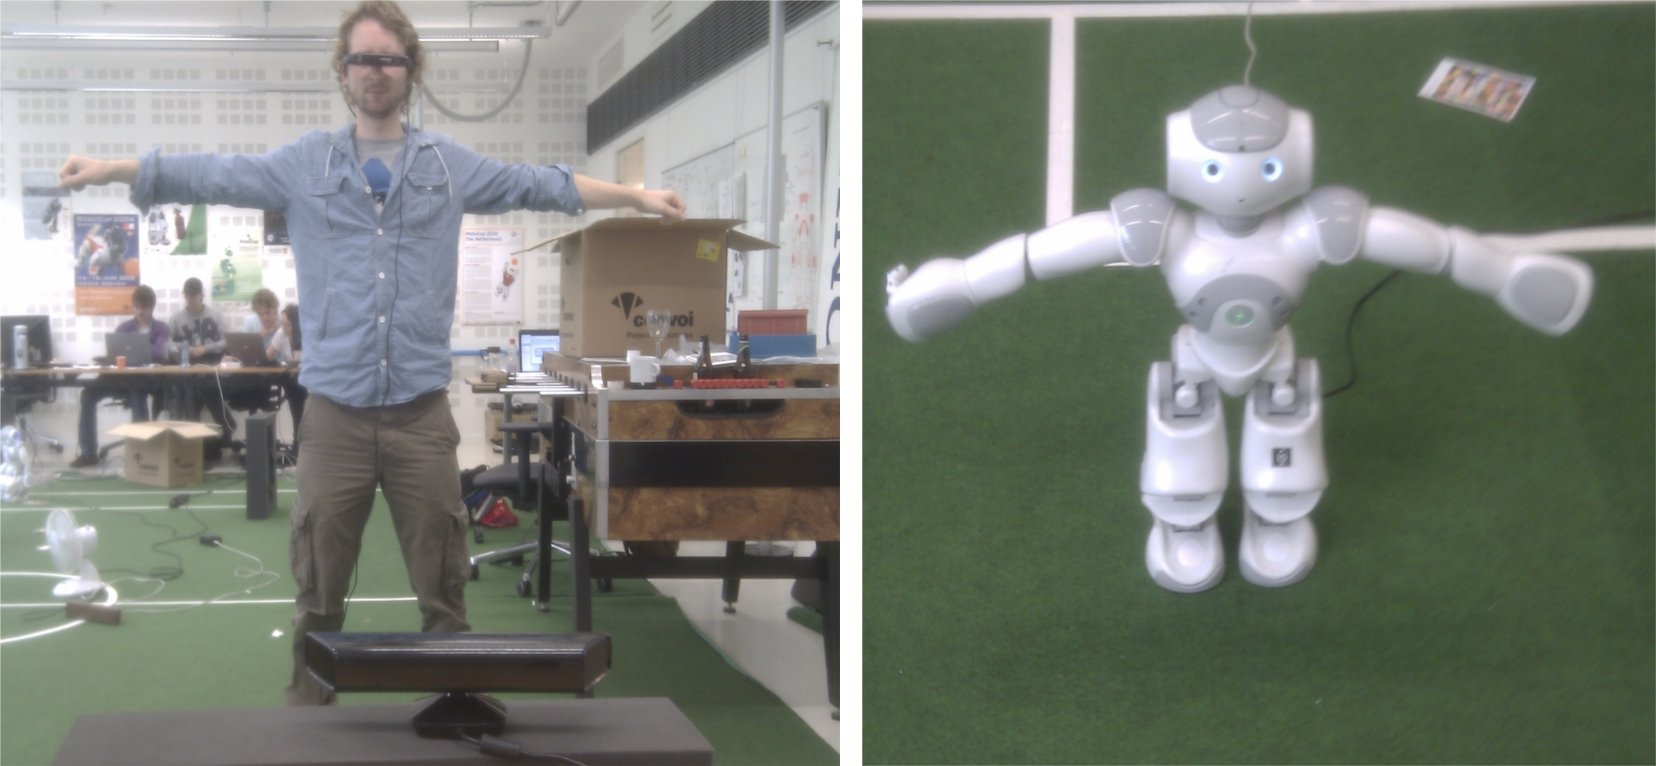
\includegraphics[width=1\columnwidth]{KiNao_Poses.jpg}}
\caption{The system in use}
\label{fig:Duncan}
\end{figure}

The system implemented allows a human user to control humanoid robots through body motions (see figure \ref{fig:Duncan}). It does not require the user to lift the legs or walk, only the upper body is mimicked. Requirements for use are perhaps a few hours of practice but no knowledge of robotics is needed. It is therefore applicable in any area. A few examples of possible use are teleoperation in dangerous area’s (e.g.\ after natural disasters or warzones), house-holding tasks but also industrial processes. The human interface makes it relatively easy to learn the robot a new task since it can simply mimic the user executing the task. This task is relevant to the RoboCup precisely because of that. While not currently possible, balancing while mimicking a human operator drastically shortens the time needed to design a motion. A user can simply execute a motion while seeing the Nao mimic it. This motion is then recorded and smoothed (removing noise due to inaccuracies by the Kinect, removing control points, etc.). This simplification of motion design makes it possible for an inexperienced (meaning no experience with Naos) user to create basic, but smooth, keyframe motions.

\section{Acknowledgements}
The Dutch Nao Team likes to thank the following people:
\begin{itemize}
\item Sander van Noort for his contribution to the simulation. 
\item The University of Amsterdam for their support, the new lab, the contributions and experience we get from this project. 
\item All our Artificial Intelligence teachers for when they took RoboCup into account.
\item Adwin Verschoor of Cena-Werk\footnote{Visit him at \url{http://www.cenawerk.nl} for computer support} providing us with full technical support. 
\item The Italian and Iranian National Committee for their hospitality and travel support
\item RoboCup Junior for a great event
\item Marthy van de Laar for her help with Public Relations
\item The Standard Platform League for blessing us with the Robocup.
\end{itemize}
Last but not least we would like to thank: Sander Latour, Patrick de Kok, Chiel Kooijmans, our parents and everybody that has helped for their contributions.
\newpage
\bibliographystyle{mystyle}
\bibliography{references}

\section{Appendix}
\subsection{Team Poster}

\fbox{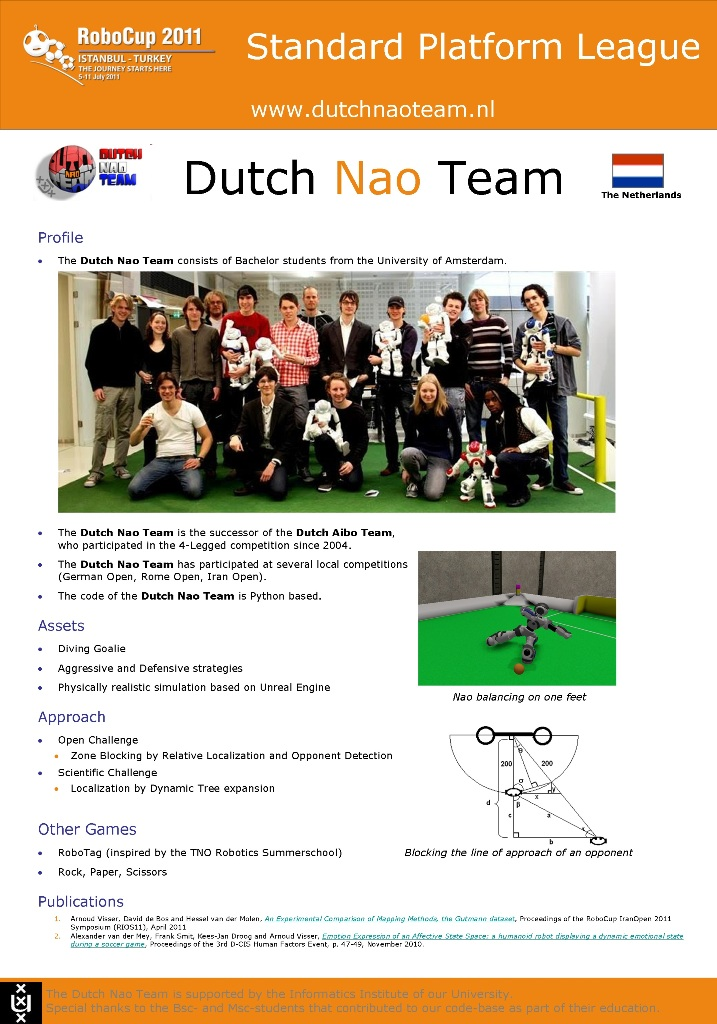
\includegraphics[height=0.9\textheight]{PosterRoboCup2011.jpg}}

\subsection{Open Challenge Document June}
\label{app:open_challenge_june}

\fbox{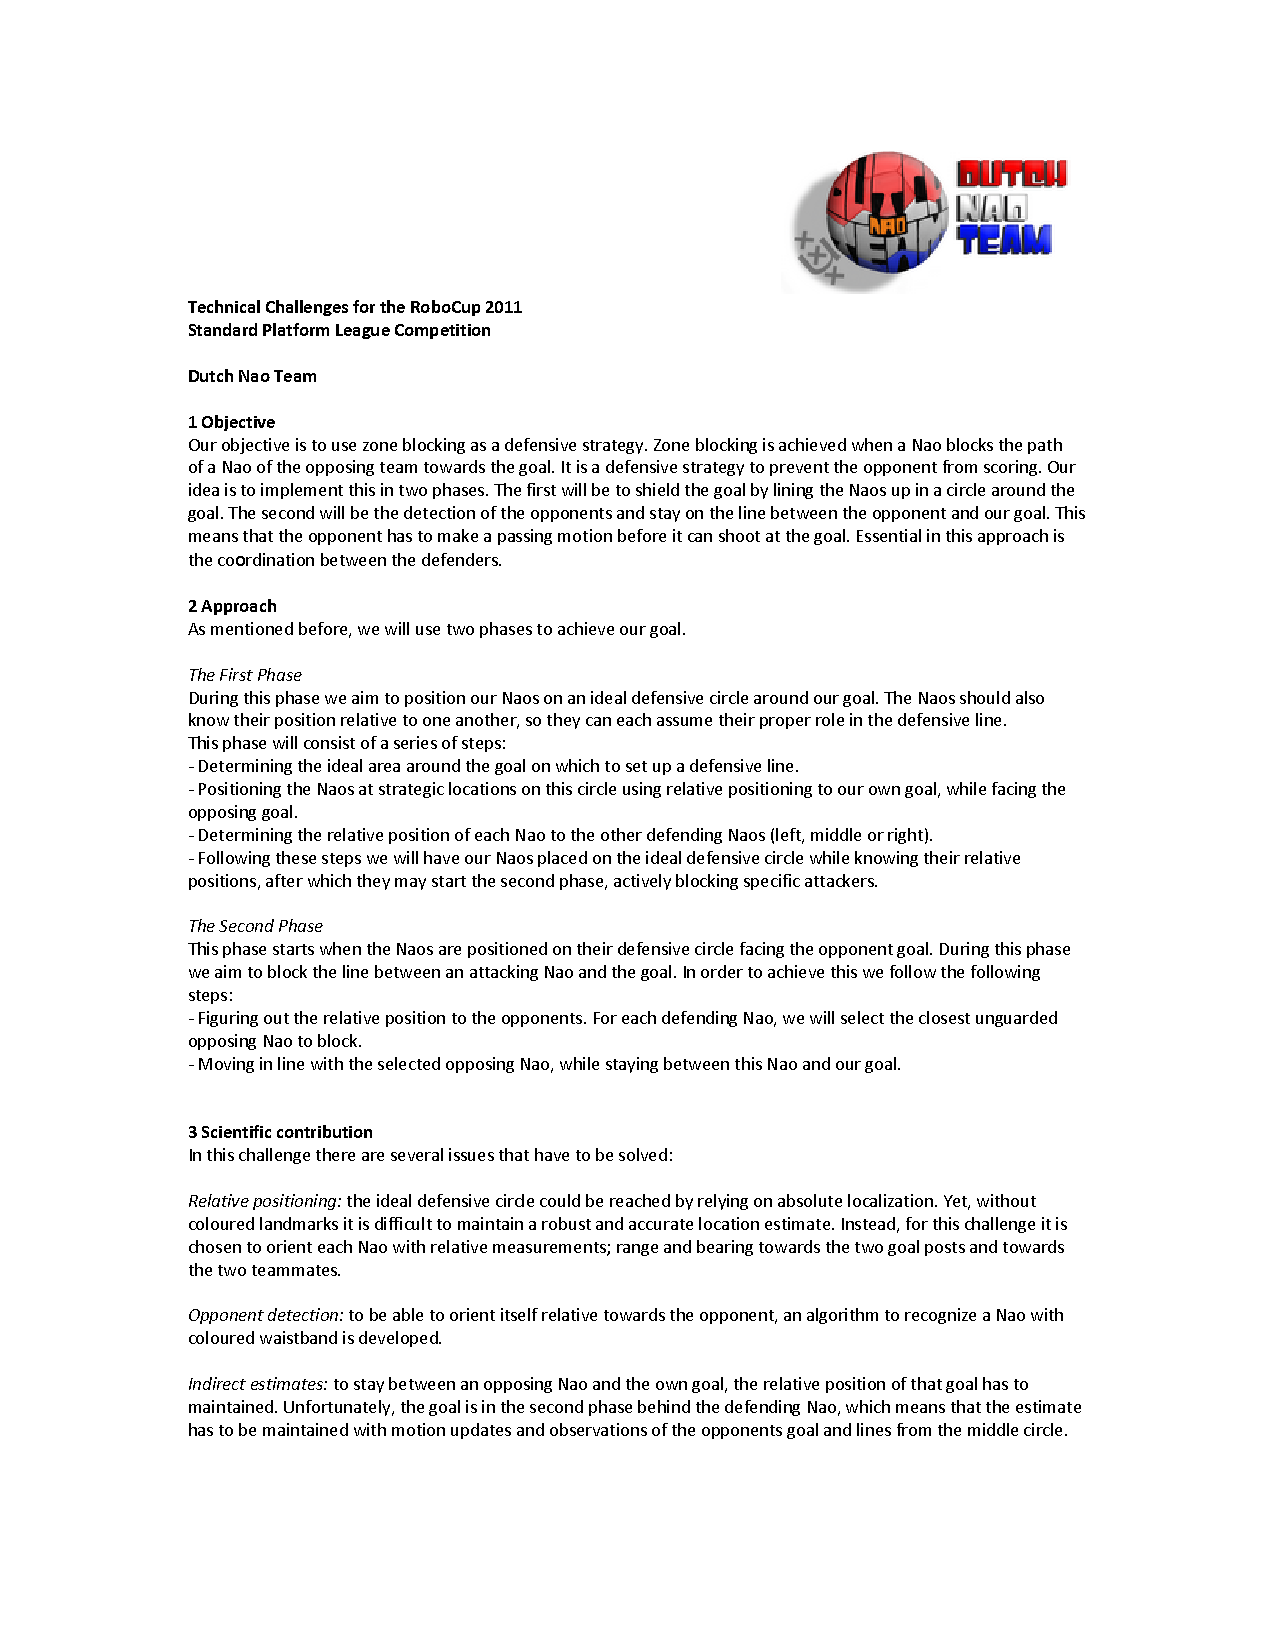
\includegraphics[height=0.9\textheight]{RoboCup2011-OpenChallengeDNT.pdf}}

\subsection{Open Challenge Document July}
\label{app:open_challenge_july}

\fbox{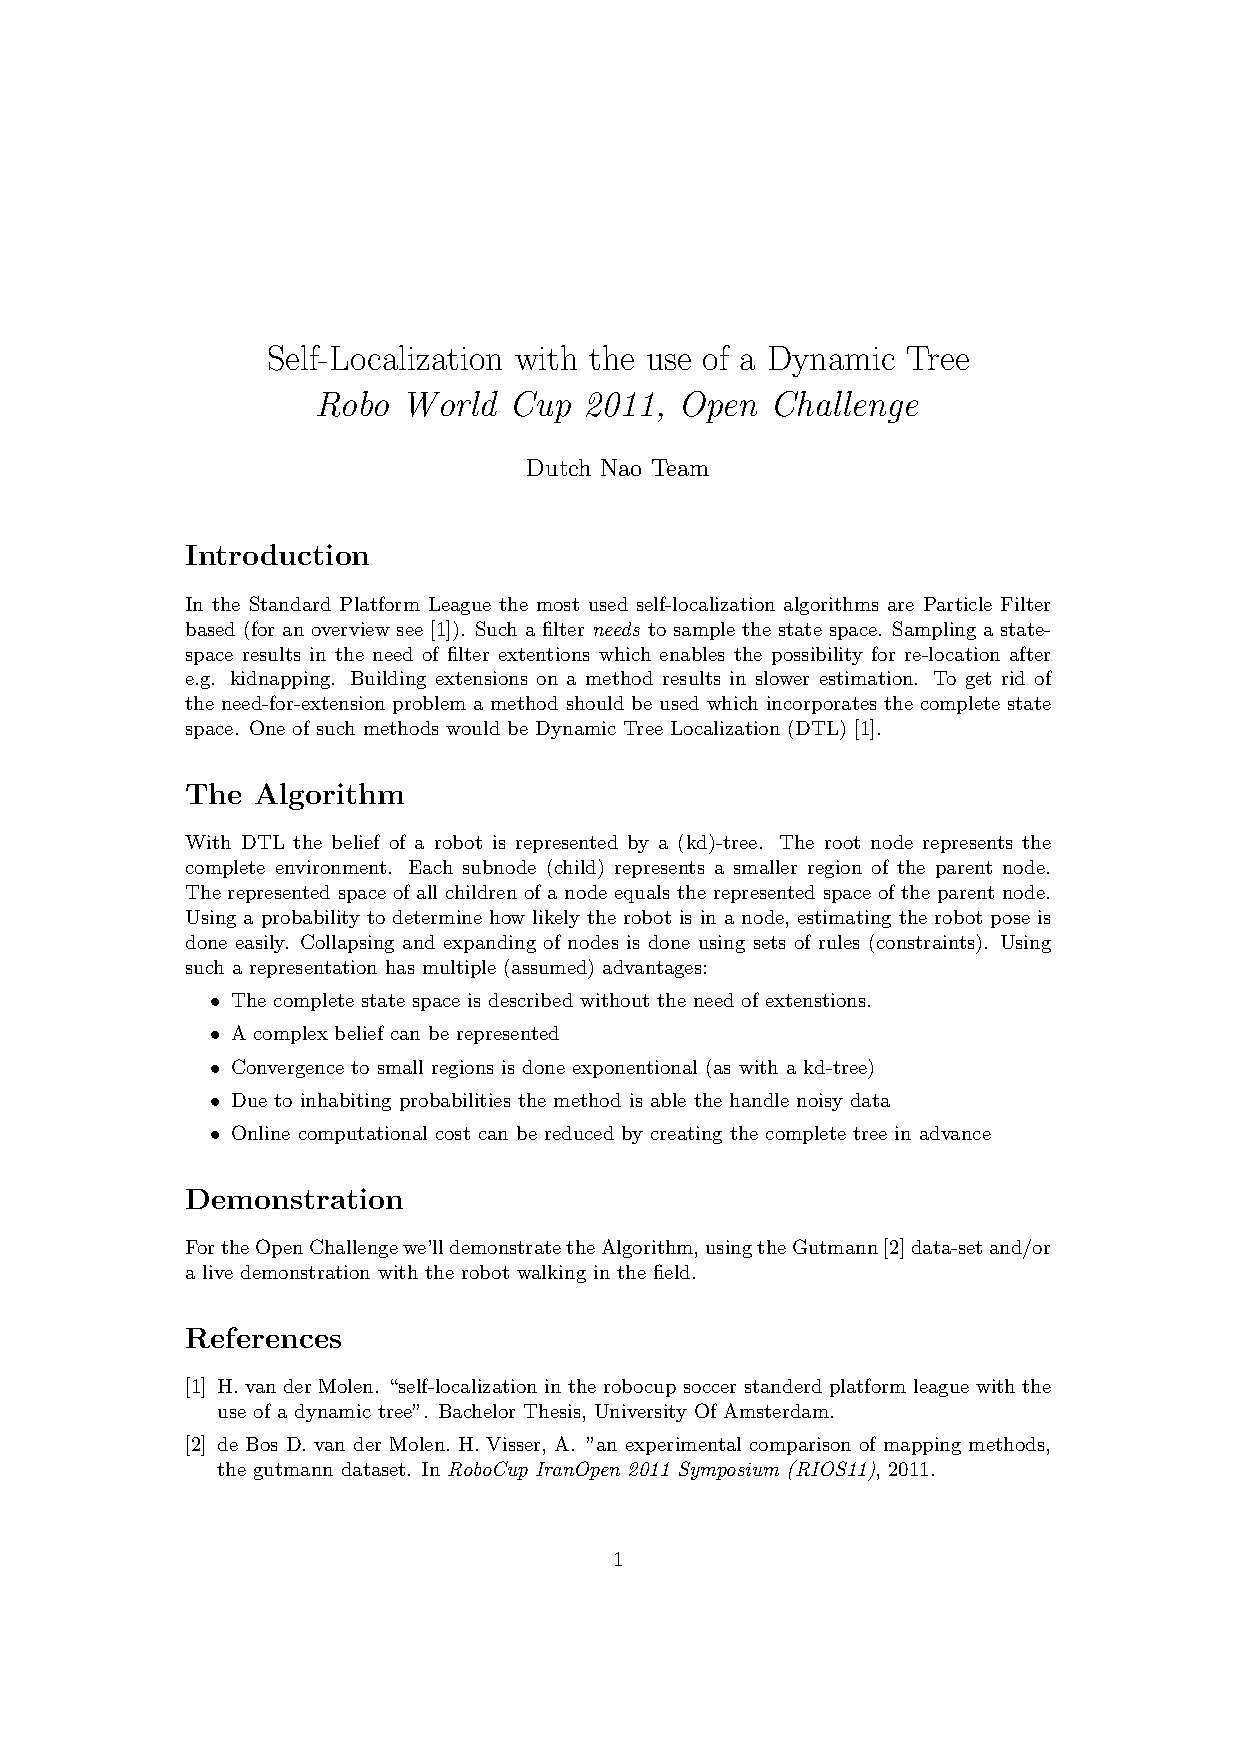
\includegraphics[height=0.9\textheight]{OpenChallenge.pdf}}

\subsection{Press release}
\label{app:press_release}
\fbox{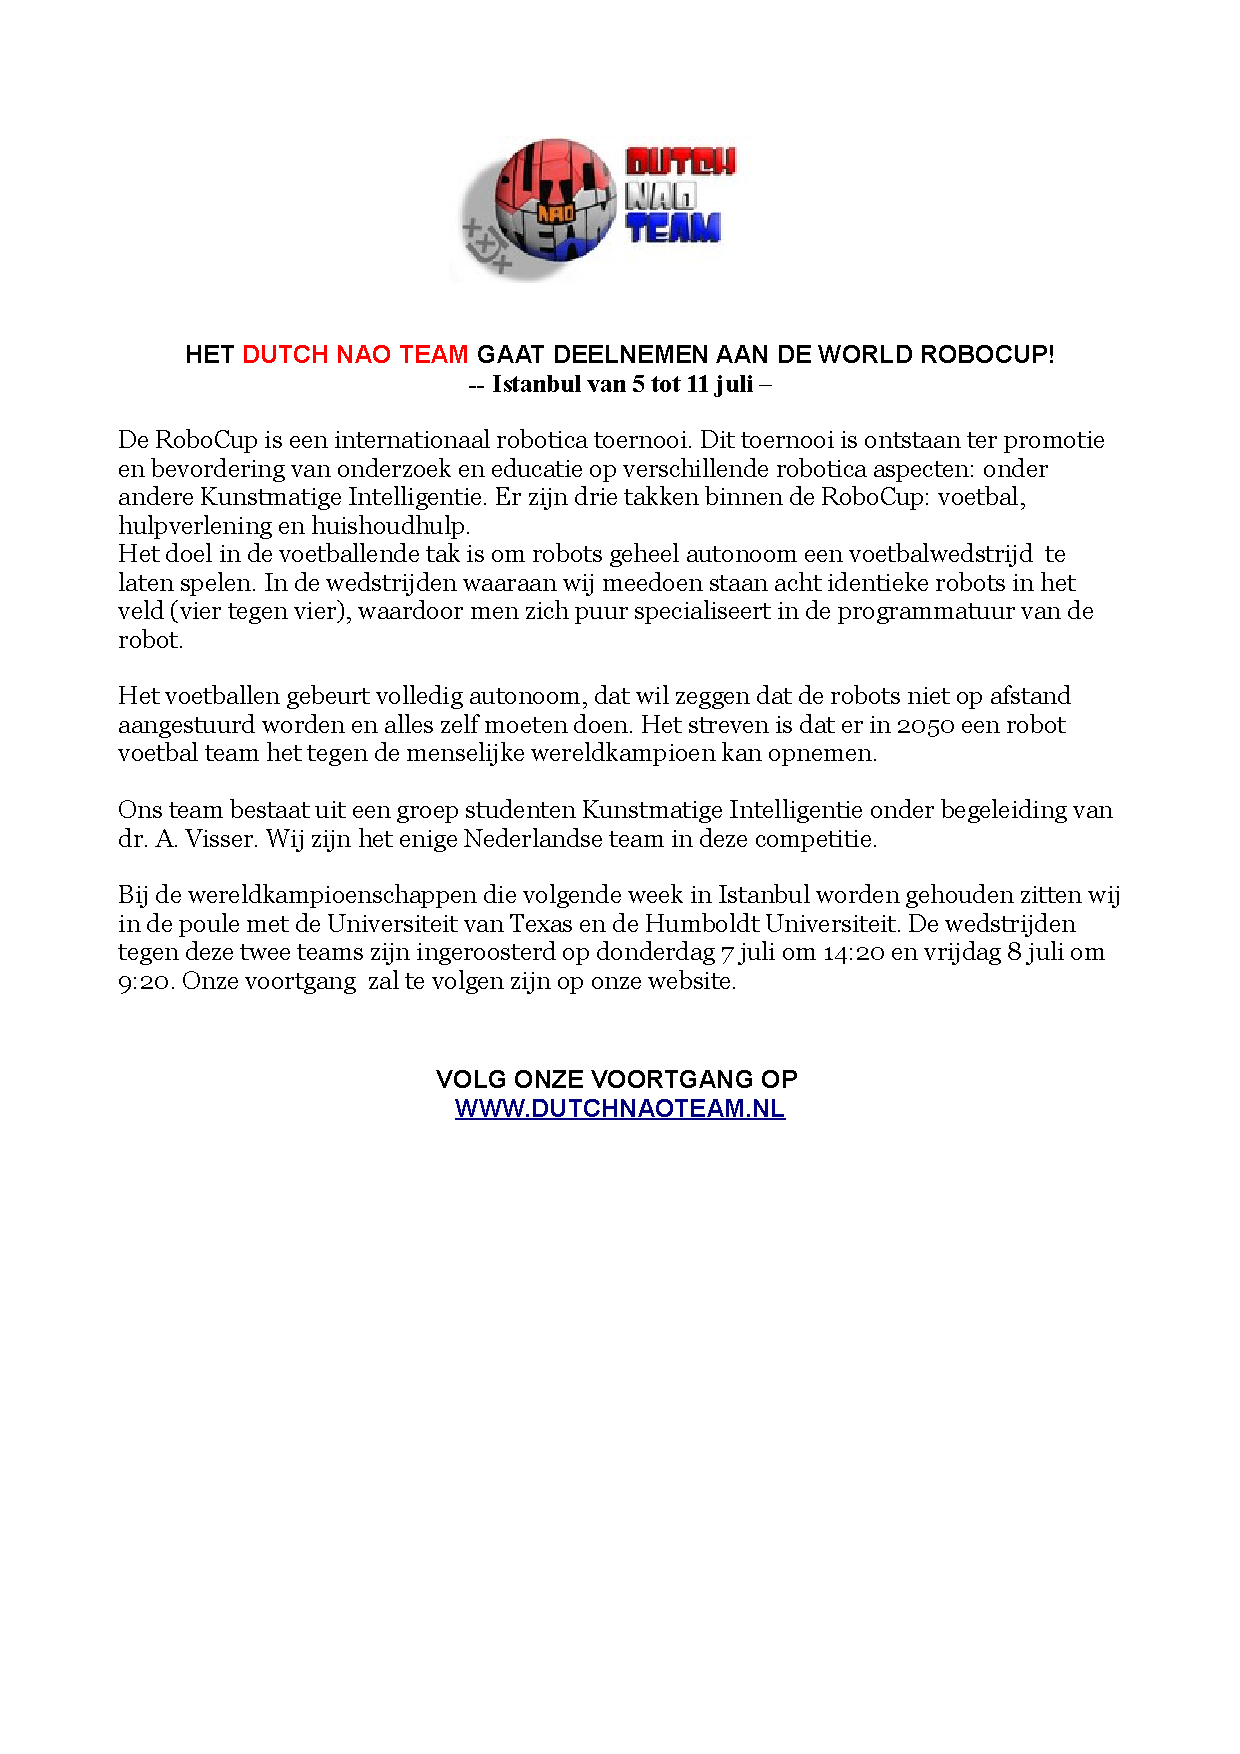
\includegraphics[height=0.85\textheight]{DNTpersbericht.pdf}}

\subsection{File Overview}
\label{app:file_overview}

\fbox{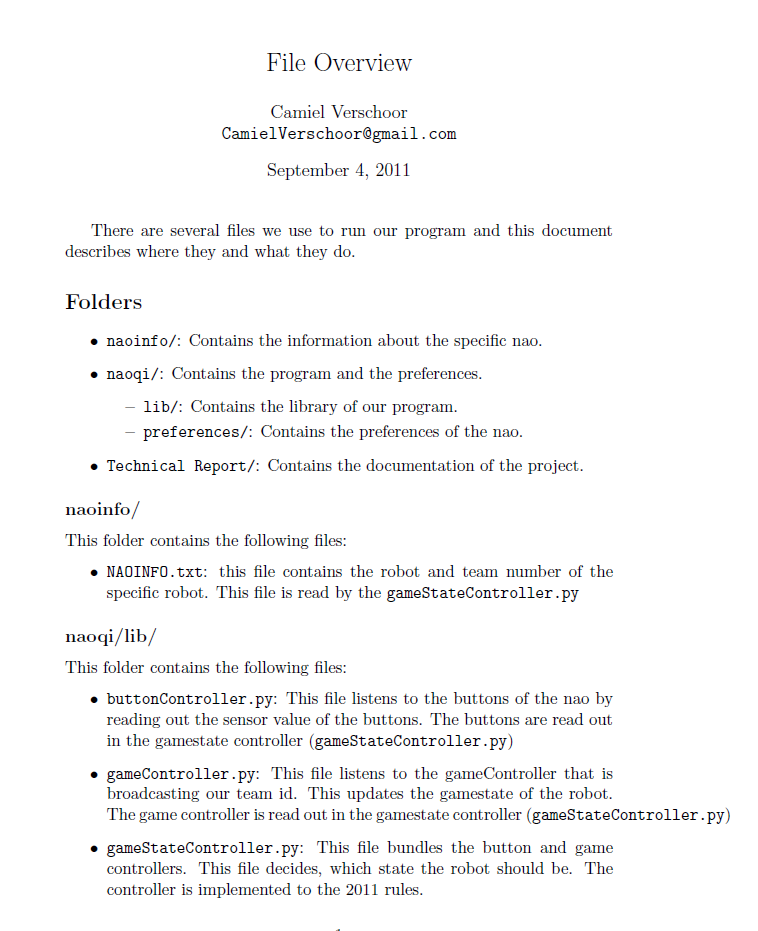
\includegraphics[width=\columnwidth]{FileOverviewPage1.png}}

\fbox{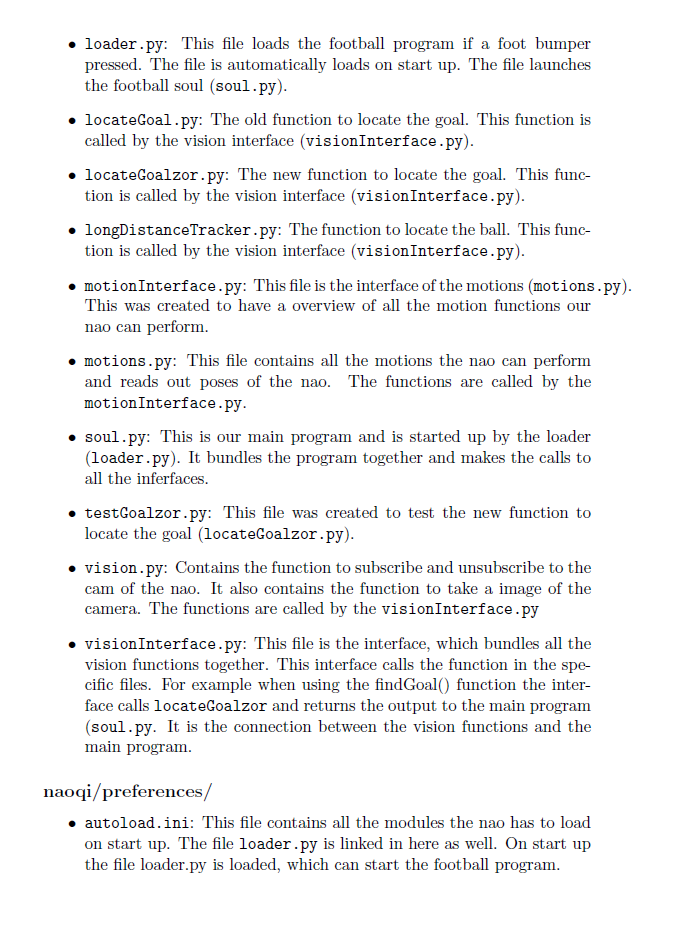
\includegraphics[width=\columnwidth]{FileOverviewPage2.png}}
\end{document}
